%%%%%%%%% PROPOSAL -- 15 pages (including Prior NSF Support)
% From the NSF Grants Proposal Guide:
% "The Project Description should provide a clear statement of the work 
% to be undertaken and must include: objectives for the period of the proposed 
% work and expected significance; relation to longer-term goals of the PI's 
% project; and relation to the present state of knowledge in the field, 
% to work in progress by the PI under other support and to work in progress 
% elsewhere."

%\required{Project Description}
\section{Project Description}

\begin{figure}[!h]
        \begin{center}
		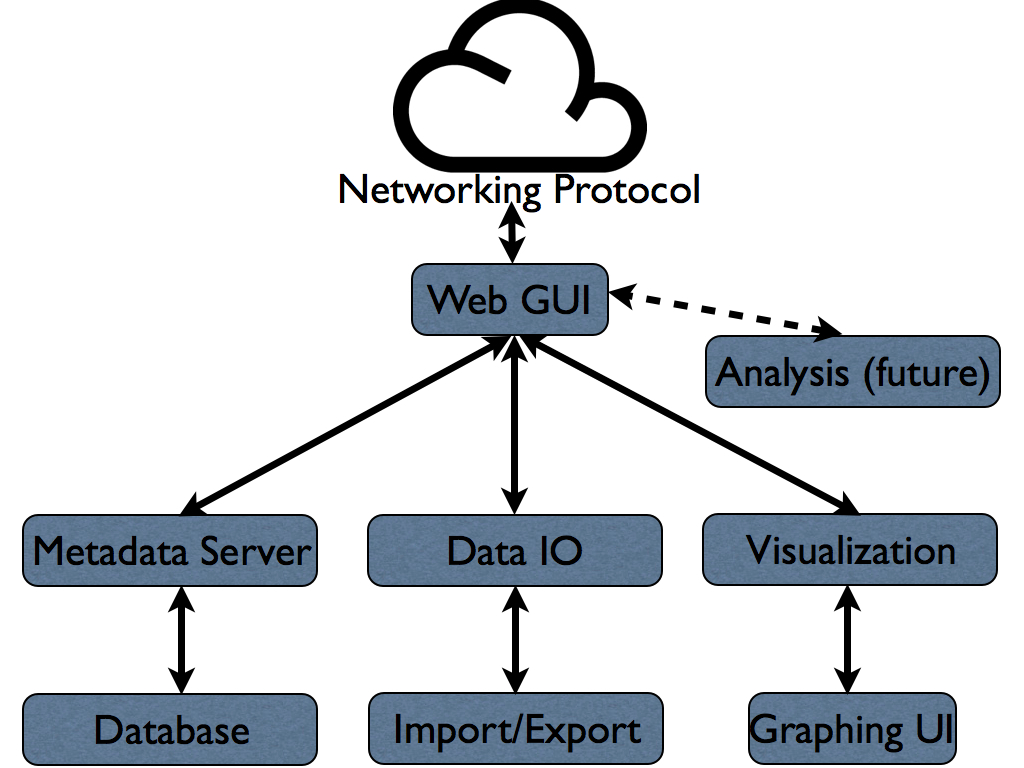
\includegraphics[width=120mm]{images/tool_layout}
                \caption{Software tool's component layout}
                \label{tool_layout}
        \end{center}
\end{figure}


\subsection{Methodology}
The team will develop the software in whatever style they like, but will report
weekly to the customer with progress reports and new project projections. 
Project leaders may occasionally travel with Alex Fremier to meet with other
users, but only optionally. Weekly trends will give projections, and a 
customer acceptance test will conclude at the end of the semester.

\subsubsection{Software Requirements}
This project will be written a web interface, preferably using a Model View
Control (MVC) Design pattern like Ruby on Rails. The web gui will implement
a RESTful interface, and will implement modules for inputing, filtering, 
visualizing, and analizing data.

The project will contain 4 different module sections:
\begin{enumerate}
	\item Metadata server and database
	\item Data input / output
	\item Visualization and selection interface
	\item Networking protocol
	\item A stub for an analysis pipeline
	%more?
\end{enumerate}

The metadata server module will allow the user to specify what format they 
will like to use (MySQL, PostGreSQL, SQLite, Casandra). It will help them
manage backups, both locally and offsite, and the scheduling of backups. It will
allow them to select which offsite datasets or entire hosts to mirror, and
help them automate the management of data collisions. The interface will also
allow them to monitor the health of offsite hosts, and view statistics
about the network health going to the host.

The data input / output modules will help users input various different
data standards (CSV, R language tables, more) into the tool's common 
metadata format, which will be similar to an SQL table format. These modules
will also allow users to apply a few useful filters to the data, similar to
how Microsoft Excel can. When an data input session start, the data will be 
staged as a sandbox dataset, and the user will be able to sort, apply filters,
and delete data similar to a spreadsheet, until the data is formatted correctly.

The data visualization and selection modules will help users with graphing
their data in an array of charts, and have spatial data represented on 
3D plots. Users will be able to select ranges from the charts, and have the
resulting datasets cached for them for future processing. Users will be able
to join multiple datasets, split datasets, and describe relations between 
different datasets. They will be able to create lookup tables between datasets
on the fly, allowing them the maximize data usability while minimizing data 
redundancy.

The networking modules will provide different ways to syncronize data. These
can utilize current network protocols, as well as try to implement new
ones. Examples of existing protocols can include rsync, http, ftp, scp, SOAP
XML, built in database protocols, and more. The data should make sense, however,
in whatever incremental state it is in. If a large transfer, or a small
transfer on a slow connection, fails, then the receiving host should see the
transfered pieces of data in a dataset, and see a visible gap (i.e. through
the visualization tools). The client can then choose to resend, and the minimal
amount of retransmits should occur to finish the transmission.

The distribution will be installable on Windows, 
Linux, and Mac, and will include any third party source needed. It will be 
downloadable to customers via a repository. 

\section{Customer}
The customer will be Alex Fremier of the UI's College of Natural Resources.
If this project proposal is accepted, specific customer requirement will be 
drawn and presented at the beginning of the Spring 2012 semester. An 
acceptance test will be specified along with a full list of function tests.

%\section{Statement of Qualifications}

%\section{Conclusion}
%Why should people pay for this thing, why should the capstone PM's want
% this project, and why is it great for humanity


%\required{Broader Impacts}
% as in the project summary, broader impacts must be called out separately 
% in the project description.  You may be able to give more specific
% examples, or discuss how you've previously achieved these impacts.
% It should be similar, but not identical, to the Broader Impacts statement
% in the project summary

%\required{Results From Prior NSF Support}
% 5 pages or fewer of the 15 pages for entire description document.
% include results from NSF grants received in the past 5 years.
% if supported by more than one grant, choose the most relevant one
% for each grant, include: NSF award number, amount, dates of
% support, and publications resulting from this research.
% due to space limitations, it is often advisable to use citations rather
% than putting the titles of the publications in the body 
% of this section

% e.g.: "My prior grant, "Uses of Coffee in Mathematical Research" (DMS-0123456, 
% $100,000, 2005-2008), resulted in 3 papers [1],[2],[3], demonstrating..."

% if requesting postdoctoral research salary, a supplemental 1-page document
% called "Postdoc Mentoring Plan" will be required 

